\documentclass{standalone}

\usepackage{tikz}
\usepackage{pgfplots}
\usetikzlibrary{positioning,fit}
\pgfplotsset{compat=newest}

\begin{document}
  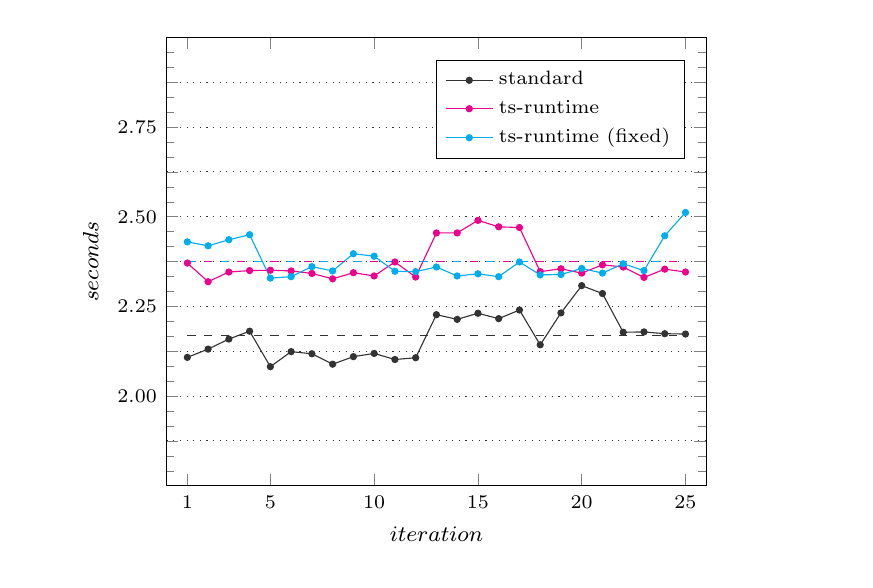
\begin{tikzpicture}[
  font=\footnotesize
  ]
  
    \tikzset{mark size=1.1}
  	\pgfplotsset{major grid style={dotted,black!80}}
  	
  	\begin{axis}[
      use as bounding box,
      ylabel style={overlay},
  		yticklabel style={overlay},
  		legend style={
  			at={(0.96,0.95),anchor=north}
          },
    		label style={font=\footnotesize},
    		tick label style={font=\scriptsize},
    		legend cell align={left},
    		minor tick num=2,
    		ymajorgrids=true,
    		xtick={1,5,10,15,20,25},
    		ytick={1.75,1.875,2.00,2.125,2.25,2.375,2.50,2.625,2.75,2.875,3.0},
    		yticklabels={,,2.00,,2.25,,2.50,,2.75,,},
    		y tick label style={
    			/pgf/number format/.cd,
    			fixed,
    			fixed zerofill,
    			precision=2
    		},
    		xlabel={$iteration$},
    		ylabel={$seconds$},
    		xmin=0,
    		xmax=26,
    		ymin=1.75,
    		ymax=3
    	];
    
  		\addlegendentry{\scriptsize{standard}}
  		\addplot[
  			color=black!80,
  			mark options={solid,black!80},
  			mark=*
  		] coordinates {
  			(1,2.108)
  			(2,2.131)
  			(3,2.159)
  			(4,2.181)
  			(5,2.082)
  			(6,2.124)
  			(7,2.118)
  			(8,2.089)
  			(9,2.110)
  			(10,2.119)
  			(11,2.102)
  			(12,2.107)
  			(13,2.227)
  			(14,2.214)
  			(15,2.231)
  			(16,2.216)
  			(17,2.240)
  			(18,2.143)
  			(19,2.232)
  			(20,2.308)
  			(21,2.286)
  			(22,2.178)
  			(23,2.179)
  			(24,2.174)
  			(25,2.173)
  		};
  		
  		\addlegendentry{\scriptsize{ts-runtime}}
  		\addplot[
  			color=magenta,
  			mark options={solid,magenta},
  			mark=*
  		] coordinates {
  			(1,2.371)
  			(2,2.319)
  			(3,2.346)
  			(4,2.350)
  			(5,2.351)
  			(6,2.349)
  			(7,2.342)
  			(8,2.327)
  			(9,2.344)
  			(10,2.335)
  			(11,2.374)
  			(12,2.332)
  			(13,2.455)
  			(14,2.455)
  			(15,2.490)
  			(16,2.472)
  			(17,2.470)
  			(18,2.347)
  			(19,2.355)
  			(20,2.343)
  			(21,2.366)
  			(22,2.360)
  			(23,2.331)
  			(24,2.354)
  			(25,2.346)
  		};
  		
  		\addlegendentry{\scriptsize{ts-runtime (fixed)}}
  		\addplot[
  			color=cyan,
  			mark options={solid,cyan},
  			mark=*
  		] coordinates {
  			(1,2.430)
  			(2,2.419)
  			(3,2.436)
  			(4,2.450)
  			(5,2.329)
  			(6,2.333)
  			(7,2.361)
  			(8,2.349)
  			(9,2.397)
  			(10,2.390)
  			(11,2.348)
  			(12,2.347)
  			(13,2.360)
  			(14,2.335)
  			(15,2.341)
  			(16,2.333)
  			(17,2.374)
  			(18,2.338)
  			(19,2.339)
  			(20,2.356)
  			(21,2.343)
  			(22,2.369)
  			(23,2.350)
  			(24,2.447)
  			(25,2.512)
  		};
      
      \draw[black!80,dashed] (axis cs: 1,2.169) -- (axis cs: 25,2.169);
		  %\draw[black!80,solid] (axis cs: 1,2.169) -- (axis cs: 25,2.169);

		  \draw[cyan, dash pattern=on 3pt off 9pt] (axis cs: 1,2.375) -- (axis cs: 25,2.375);
		  \draw[magenta, dash pattern=on 3pt off 9pt, dash phase=-6pt] (axis cs: 1,2.375) -- (axis cs: 25,2.375);
		
		  %\draw[cyan, dash pattern=on 5pt off 5pt] (axis cs: 1,2.375) -- (axis cs: 25,2.375);
		  %\draw[magenta, dash pattern=on 5pt off 5pt, dash phase=-5pt] (axis cs: 1,2.375) -- (axis cs: 25,2.375);
  	
  	\end{axis}
    
    \node[
      draw=none,
      %minimum width=\textwidth,
      fit=(current bounding box.north west) (current bounding box.south east),
      inner xsep=5em
    ] at (current bounding box.center){};
  
  \end{tikzpicture}
\end{document}